\documentclass[aspectratio=169]{beamer}
\usepackage{multicol}
\usepackage{qrcode}
\usepackage{datetime}
\usepackage{hyperref}
\usepackage{xcolor}
\usepackage{tikz}

\usetheme{Antibes}
\setbeamertemplate{footline}[frame number]{}

\newcommand{\makemycolor}[2]{%
    \pgfmathsetmacro{\hue}{(#1/100)^1.715*0.79}%
    \definecolor{myhsbcolor}{hsb}{\hue,1,1}%
    \textcolor{myhsbcolor}{#2}%
}

\hypersetup{
    colorlinks=true,
    linkcolor=blue,
    filecolor=magenta,      
    urlcolor=blue,
    pdftitle={La Blockchain},
    pdfpagemode=FullScreen,
    }

\urlstyle{same}

\title{La Blockchain} 
\author{Valerio Vaccaro}
\newdate{date}{29}{02}{2024}
\date{\displaydate{date}}
\logo{}

\begin{document}

\begin{frame}[plain,noframenumbering]
    \titlepage
    \begin{center}
        
\includegraphics[height=1cm]{logo.png}
    \end{center}
\end{frame}

\begin{frame}[noframenumbering]
    \tableofcontents
\end{frame}

\begin{frame}{Meme}
    \begin{center}
        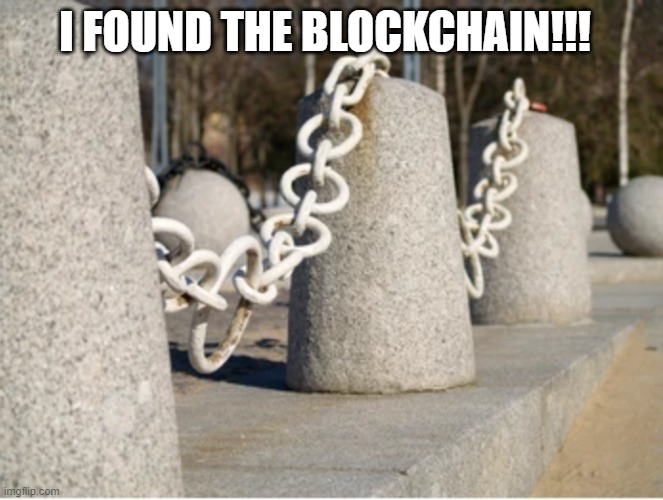
\includegraphics[height=5cm]{meme_2.jpg}
    \end{center}
    * entro la fine del corso capirete tutti i meme.
\end{frame}

\begin{frame}{Riassunto}
    Nella scorsa lezione abbiamo parlato di:
    \begin{itemize}
        \item Cosa è Bitcoin
        \item Caratteristiche e funzionalità di un nodo 
        \item Full node, SPV, Bloom Filters
        \item Tor e transportv2
        \item Mempool
    \end{itemize}
    Oggi invece approfondiremo cosa è la \makemycolor{0}{blockchain}.
\end{frame}

\section{Struttura del Blocco}

\begin{frame}{Definizione}
    La blockchain è strutturata come un’\makemycolor{0}{ordinata} \makemycolor{30}{lista di blocchi} di transazioni
    \makemycolor{0}{back-linked} ovvero in cui ogni blocco è collegato al blocco precedente.
    \begin{center}
        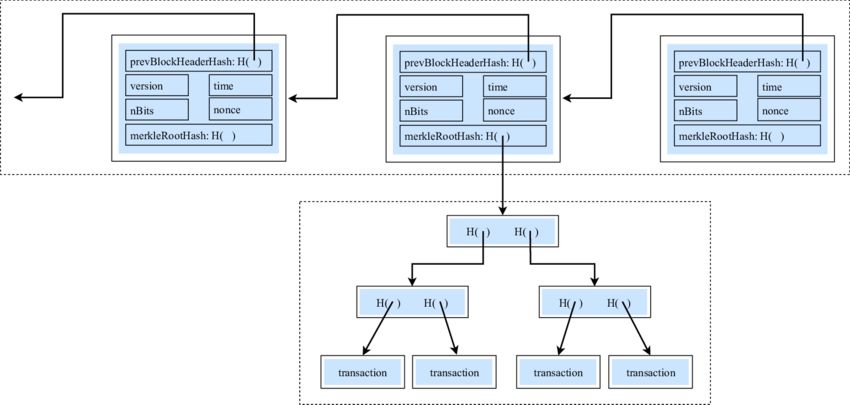
\includegraphics[height=5cm]{blockchain.png}
    \end{center}
\end{frame}

\begin{frame}{La catena}
    La catena è sempre una?

    Che succede se due miner trovano un blocco nello stesso istante?

    In Bitcoin conta il \makemycolor{0}{lavoro} fatto all'interno di un blocco.

    (Se il fork è dettato da una modifica al consenso questo split potrebbe essere insanabile!)
\end{frame}

\begin{frame}{Come è fatto un blocco?}
    \begin{center}
        Il blocco ha questa struttura:
        \begin{tabular}{|l|l|l|}
            \hline
                Dimensioni & Campo & Descrizione \\ 
            \hline
                4 byte & Block Size & La dimensione del blocco in byte\\ 
            \hline
                80 byte & Header & Campi dell'header del blocco\\ 
            \hline
                1-9 byte & Transaction Counter & Numero di transazioni presenti nel blocco\\ 
            \hline
                Variabile & Transactions & Transazioni registrate nel blocco\\ 
            \hline
        \end{tabular}
    \end{center}
\end{frame}

\begin{frame}{Header}
    \begin{center}
        L'header del blocco (80 byte) ha questa struttura:
        \begin{tabular}{|l|l|l|}
            \hline
                Dimensioni & Campo & Descrizione \\ 
            \hline
                4 byte & Version & Numero di versione del protocollo\\ 
            \hline
                32 byte & Previous Block Hash & Hash del blocco precendete (block id)\\ 
            \hline
                32 byte & Merkle Root & Radice dell'albero di merkle delle transazioni\\ 
            \hline
                4 byte & Timestamp & Orario del blocco (approssimato)\\ 
            \hline
                4 byte & Difficulty Target & Target dell'algoritmo di mining\\ 
            \hline
                4 byte & Nonce & Campo usato per il mining (ormai è troppo piccolo)\\ 
            \hline
        \end{tabular}
    \end{center}
\end{frame}

\begin{frame}{Riassumendo}
    \begin{center}
        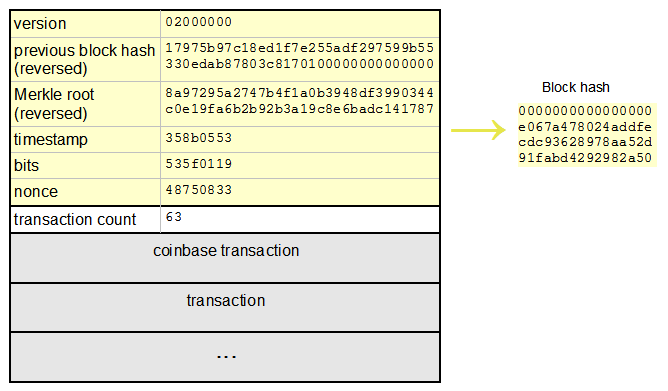
\includegraphics[height=5cm]{blocco_struct.png}
    \end{center}
\end{frame}

\begin{frame}{Altezza o identificativo del blocco?}
    L'altezza non è un dato univoco mentre lo è il block id che è ottenibile come hash (SHA256) dell'header del blocco.
    \begin{center}
        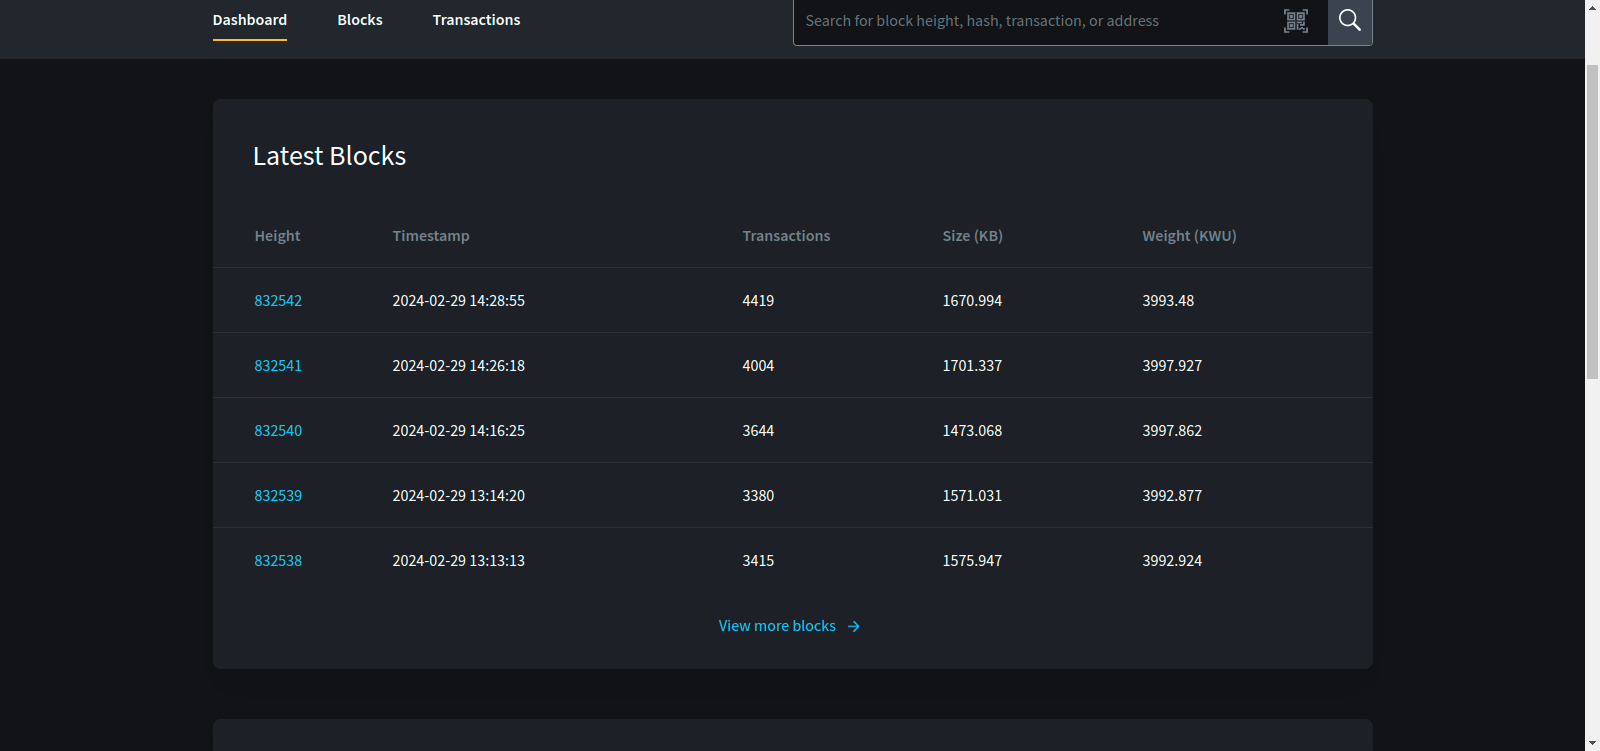
\includegraphics[height=5cm]{altezza.png}
    \end{center}
\end{frame}

\begin{frame}{Altezza o identificativo del blocco?}
    L'altezza non è un dato univoco mentre lo è il block id che è ottenibile come hash (SHA256) dell'header del blocco.
    \begin{center}
        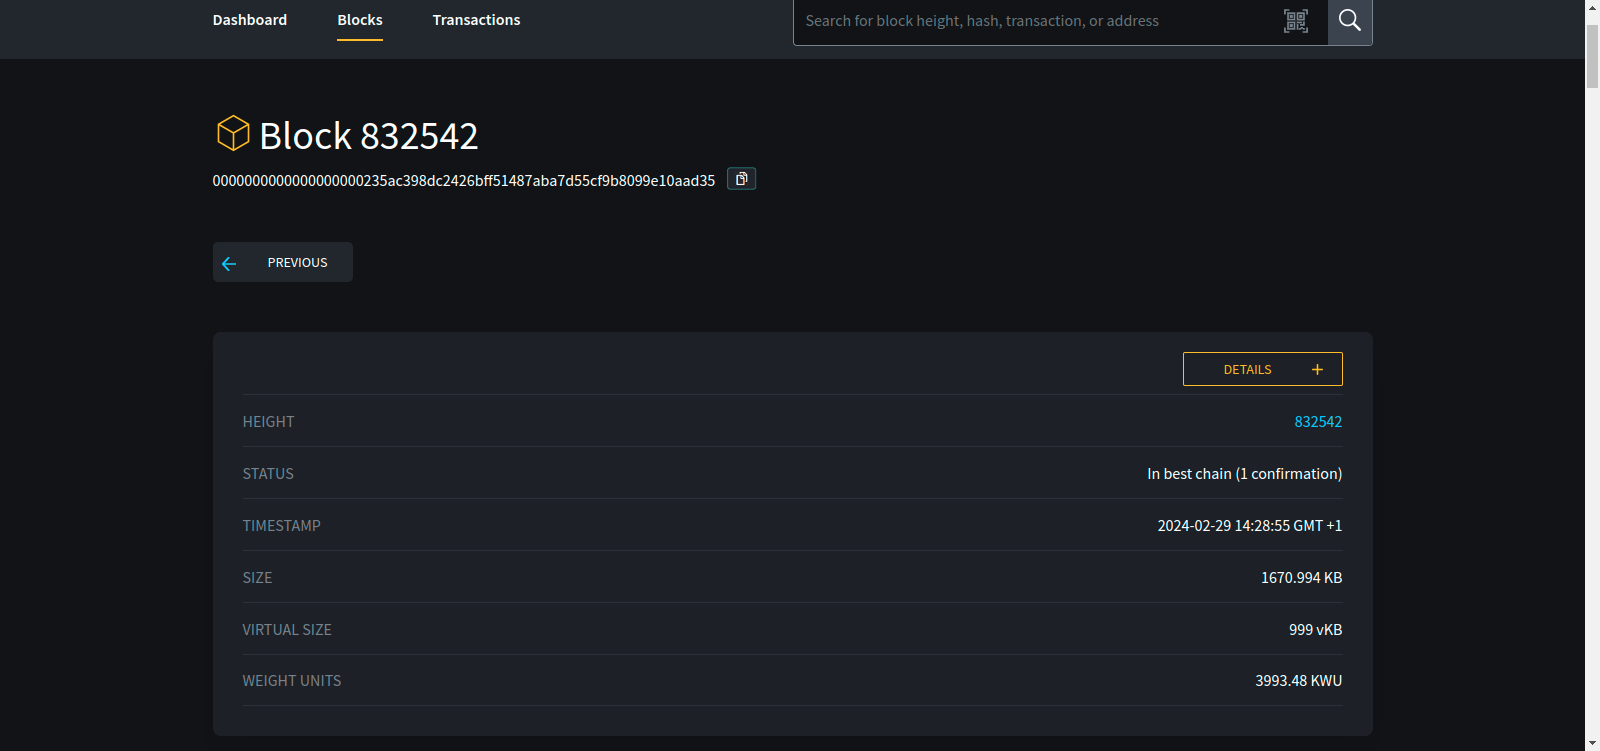
\includegraphics[height=5cm]{blockid.png}
    \end{center}
\end{frame}

\begin{frame}{Merkle tree}
    \begin{center}
        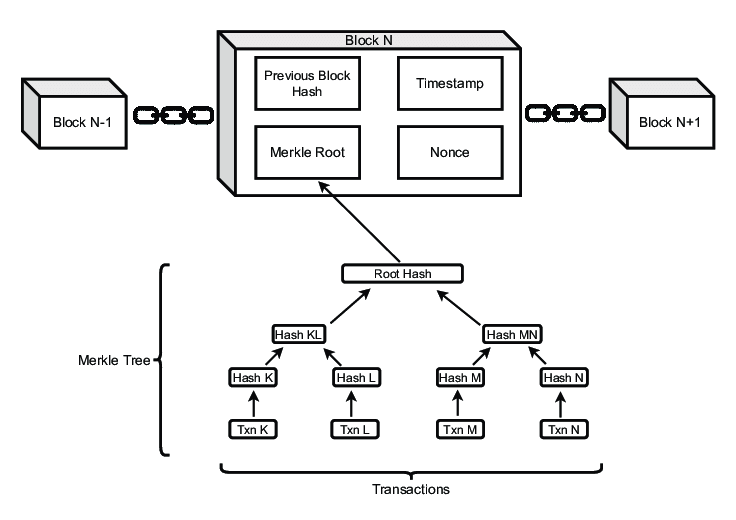
\includegraphics[height=5cm]{merkle.png}
    \end{center}
\end{frame}

\begin{frame}{Merkle tree}
   \begin{center}
        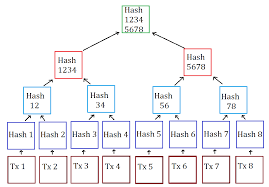
\includegraphics[height=5cm]{merkle_2.png}
    \end{center}
\end{frame}

\begin{frame}{Pausa}
    \begin{center}
        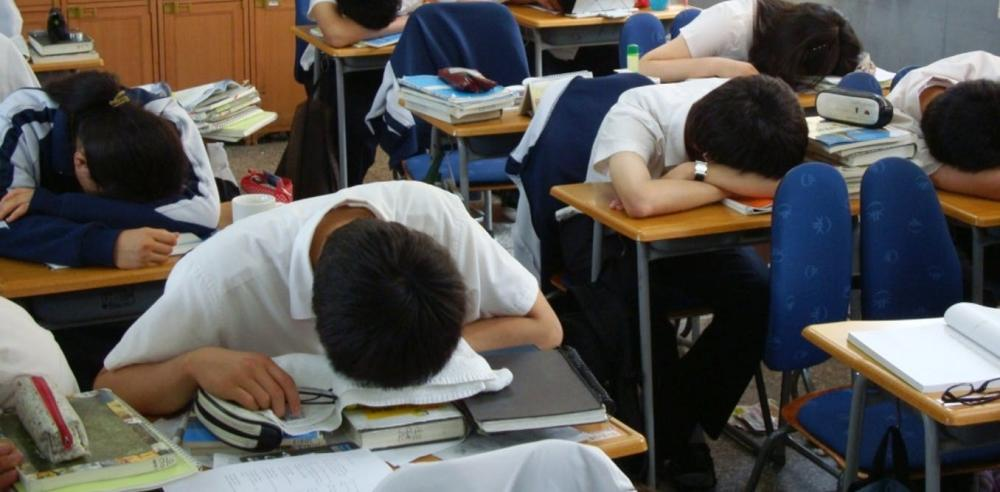
\includegraphics[height=5cm]{pausa.jpg}
    \end{center}
\end{frame}

\section{Genesis Block: analisi approfondita e particolarità}

\begin{frame}{Genesis Block}
    Blocco zero o 000000000019d6689c085ae165831e934ff763ae46a2a6c172b3f1b60a8ce26f.
    \begin{center}
        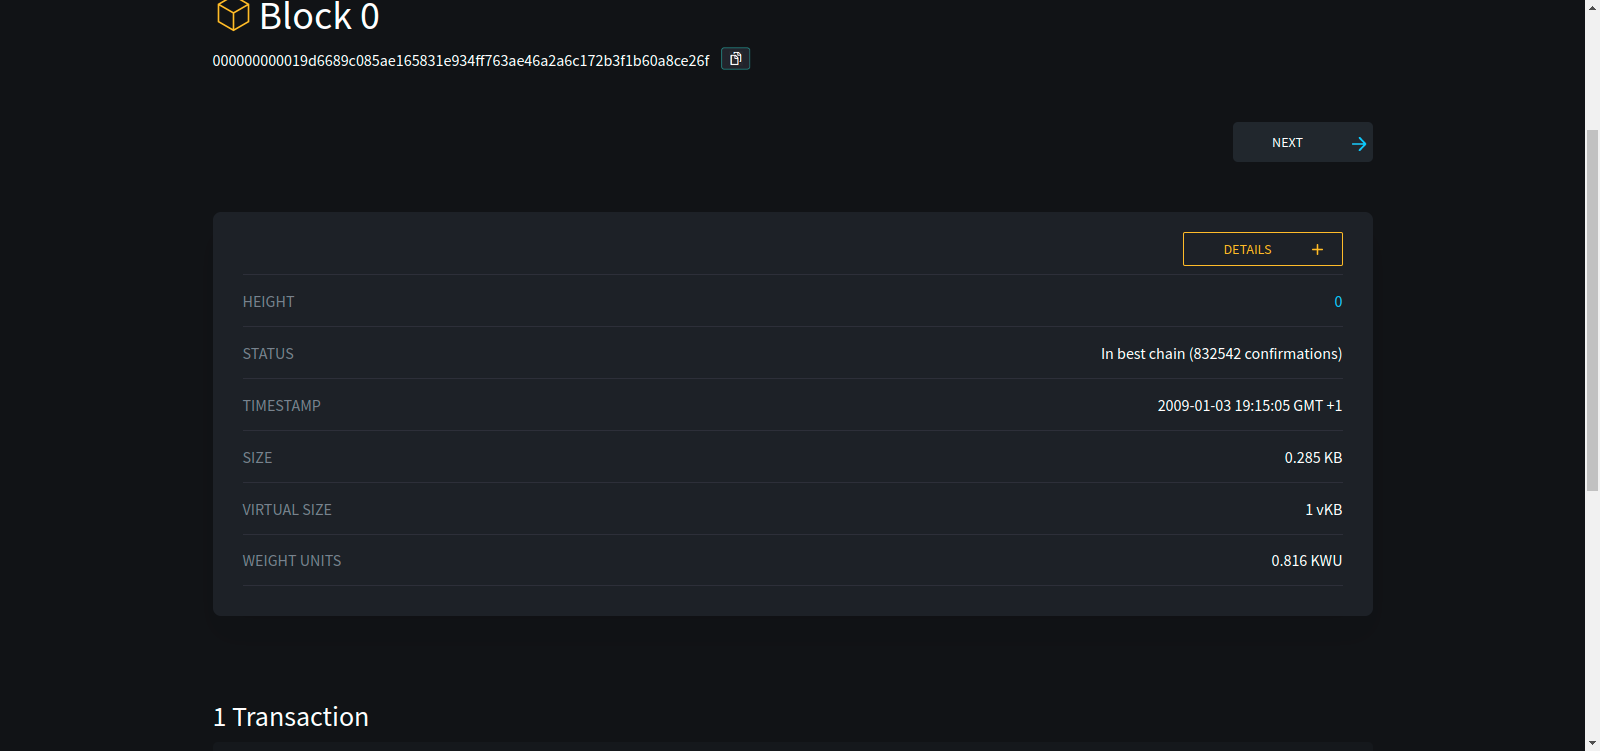
\includegraphics[height=5cm]{primo_blocco.png}
    \end{center}
\end{frame}

\begin{frame}{Coinbase}
    La prima transazione (inspendibile).
    \begin{center}
        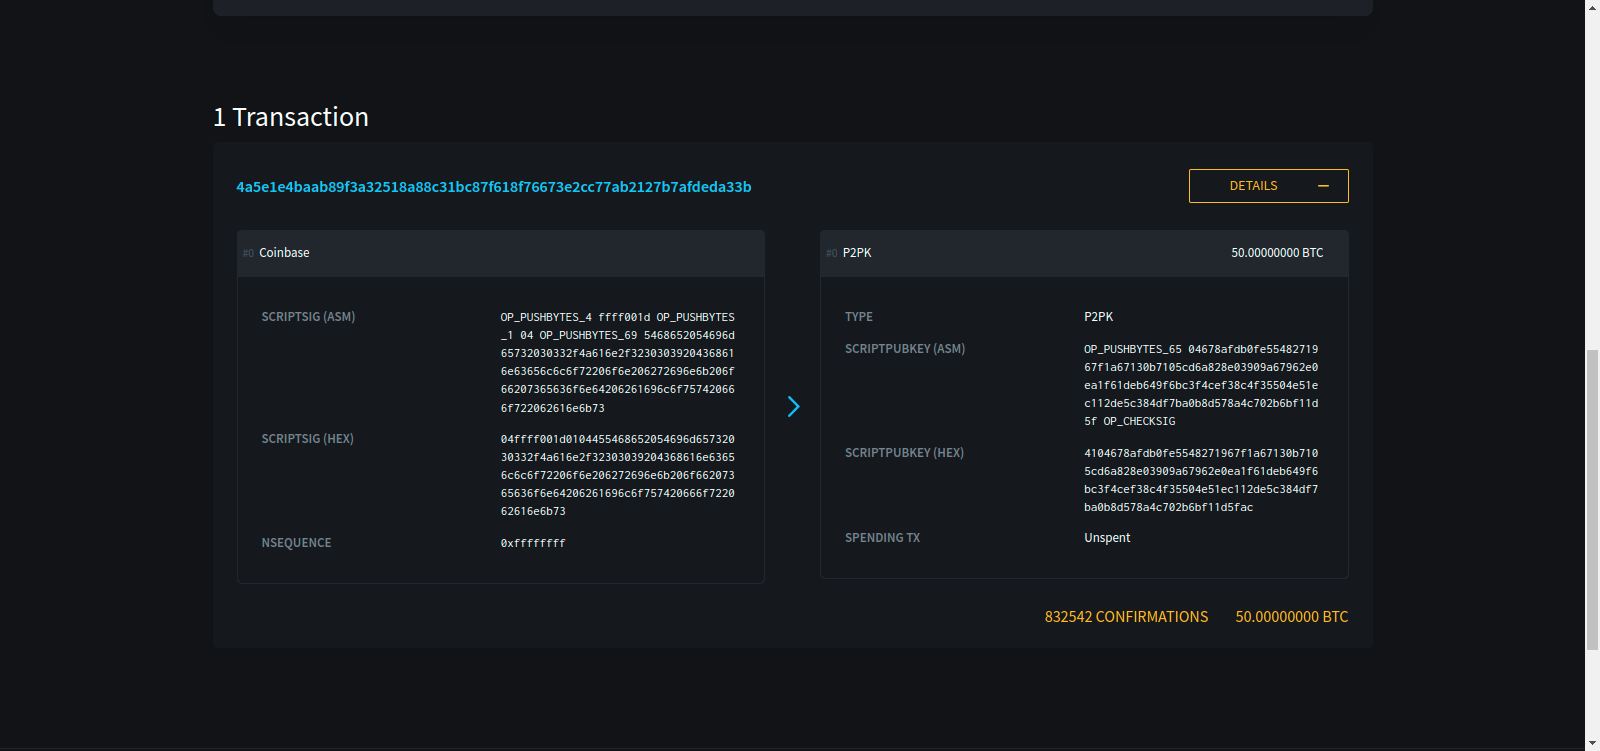
\includegraphics[height=5cm]{coinbase.png}
    \end{center}
\end{frame}

\begin{frame}{Coinbase}
    Una nota di colore ...
    \begin{center}
        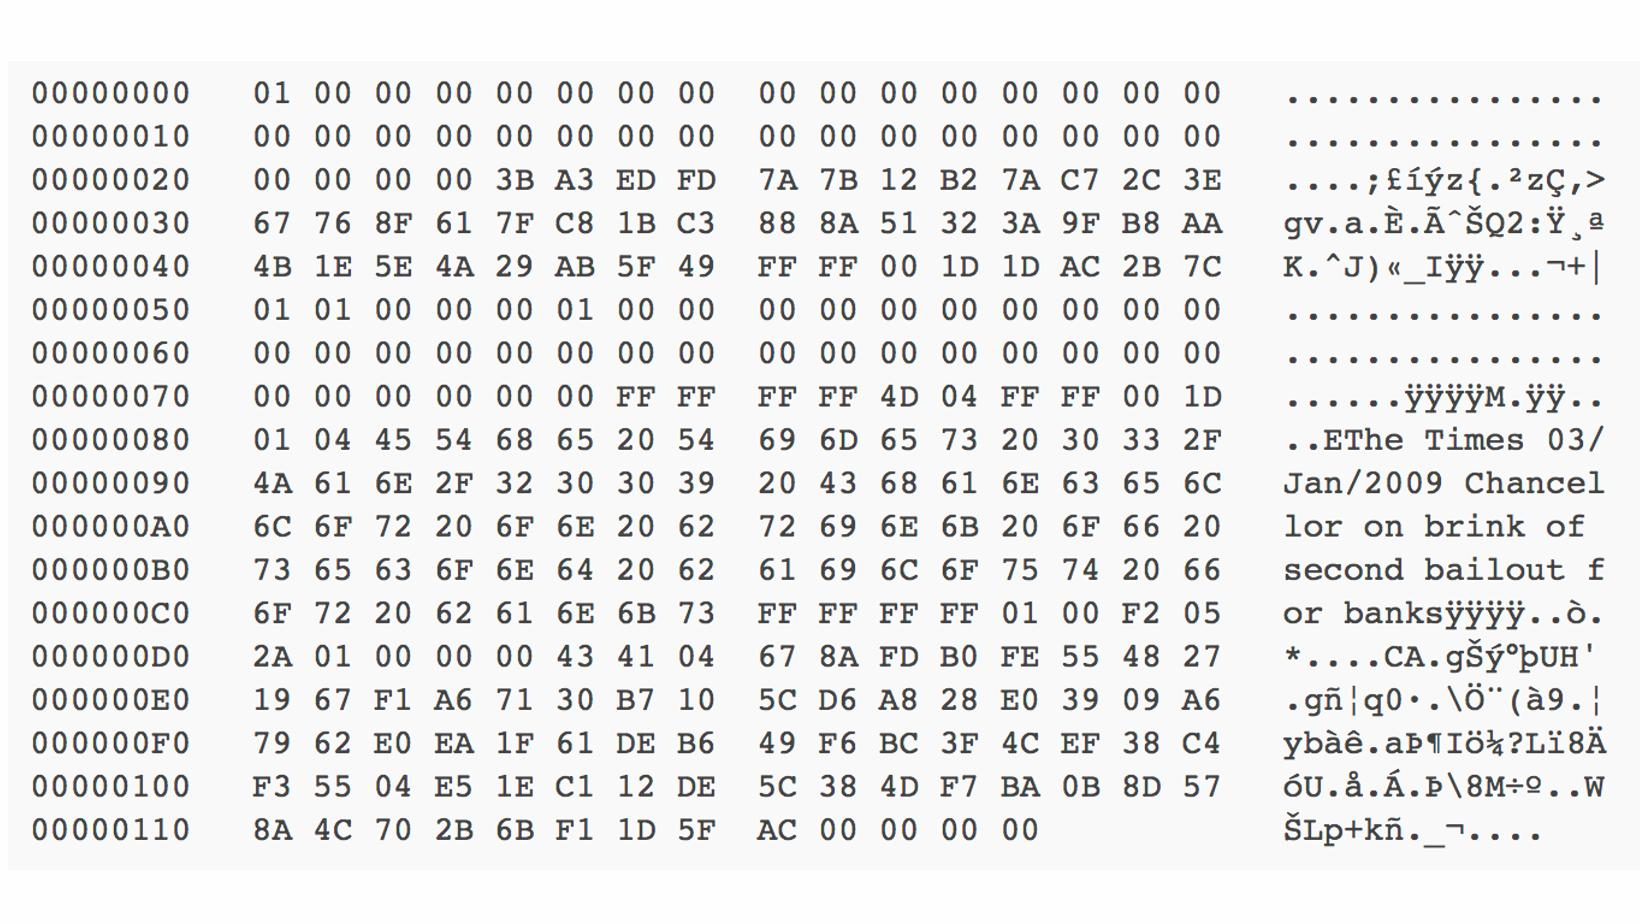
\includegraphics[height=5cm]{raw.jpg}
    \end{center}
\end{frame}

\begin{frame}{Coinbase}
    \begin{center}
        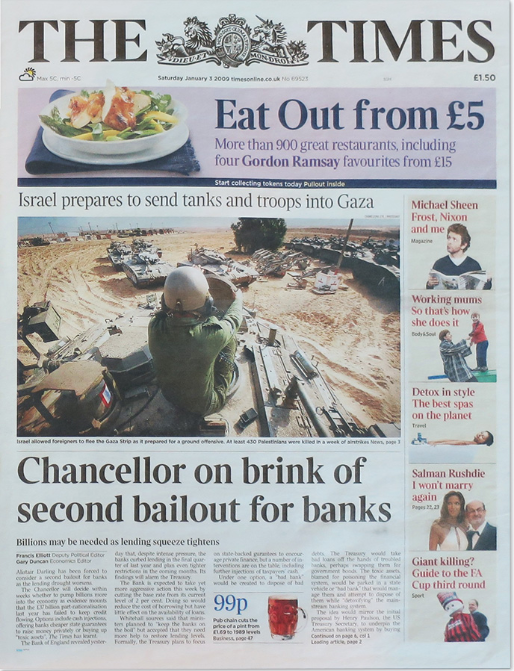
\includegraphics[height=5cm]{times.png}
    \end{center}
\end{frame}

\section{Le Blockchain di test di Bitcoin}

\begin{frame}{Introduzione}
    Per provare non serve usere per forza bitcoin in main net ma ci sono delle "istanze" alternative della blockchain utilizzatibili.

    Tali reti sono state introdotte per dare la possibilità di testate software/procedure e per scopi didattici, le principali reti sono 3:
    \begin{itemize}
        \item Testnet
        \item Signet
        \item Regtest
    \end{itemize}


\end{frame}

\begin{frame}{Testnet}
    \begin{itemize}
        \item I token hanno valore ZERO
        \item I blocchi sono generati con la stessa POW di Bitcoin
        \item Dopo 20 minuti senza blocchi la difficoltà precipita
        \item Tanti/troppi blocchi orfani
        \item Token quasi introvabili
        \item Molti wallet supportano testnet e ci sono servizi utili
        \item Ci sono molti wallet e block explorer che supportano testnet
    \end{itemize}

\end{frame}

\begin{frame}{Signet}
    \begin{itemize}
        \item I token hanno valore ZERO
        \item I blocchi sono firmati da una autorità (e sono regolari)
        \item Tanti token disponibili
        \item Poco usata
        \item Se l'autorità dovesse sparire ...
    \end{itemize}
\end{frame}

\begin{frame}{Regtest}
    \begin{itemize}
        \item I token hanno valore ZERO
        \item Voi siete Satoshi 
        \item Avete già 21.000.000 di token
        \item Minate con un comando (o anche con un miner)
        \item Non ci sono vincoli temporali sui blocchi
        \item Ovviamente vale solo sul vostro computer
        \item Facile cancellare tutto e simulare scenari complessi (ideale per CI)
    \end{itemize}
\end{frame}

\begin{frame}{}
    \begin{center}
        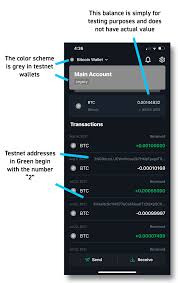
\includegraphics[height=5cm]{testnet.jpeg}
    \end{center}
    Blockstream Green supporta testnet ed è disponibile per Android, iOS, Windows, Linux e MACOS.
\end{frame}

\section{Bibliografia}

\begin{frame}{Bibliografia} 
    \begin{itemize}
        \item Andreas M. Antonopoulos, "Mastering Bitcoin", 2015
        \item Adam Back, "Hashcash-a denial of service counter-measure", 2002
        \item Satoshi Nakamoto, "Bitcoin: A Peer-to-Peer Electronic Cash System", 2008
        \item Hal Finney, "Reusable Proofs of Work", 2004
    \end{itemize}
\end{frame}

\begin{frame}{Altre risorse} 
Tra le altre risorse utili mi piace citare:
    \begin{itemize}
        \item Ovviamente \href{https://t.me/BitPolimi}{BitPolimi} che ha organizzato queste lezioni.
        \item \href{http://satoshispritz.it}{Satoshi Spritz} - eventi serali a scadenze regolari per parlare di Bitcoin (a Milano ci incontriamo ogni mercoledì dalle 18).
        \item \href{https://t.me/ventunobtc}{Ventuno} - Podcast, raccolta di libri e materiali su Bitcoin.
        \item \href{http://officinebitcoin.it}{Officine Bitcoin} - lezioni su telegram da 30 minuti per la risoluzione di problemi pratici.
    \end{itemize}
\end{frame}


\begin{frame}{Domande} 
    \begin{center}
        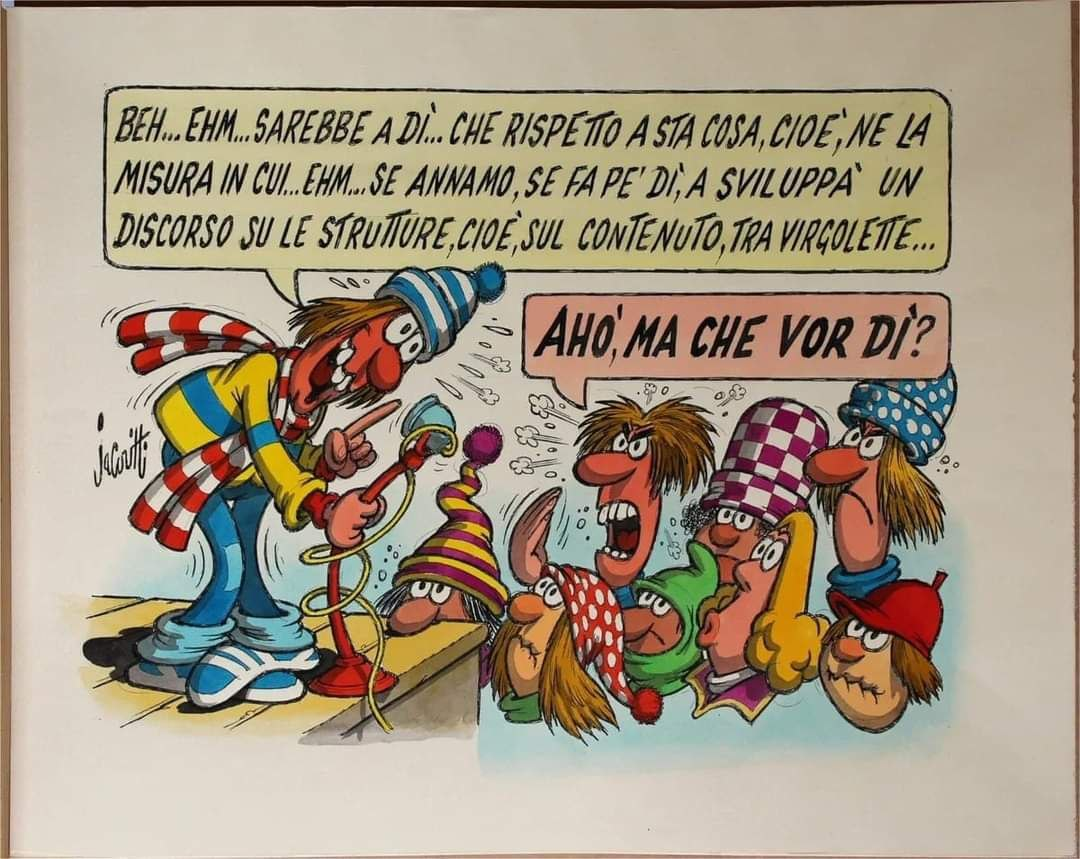
\includegraphics[height=5cm]{domande.jpg}
    \end{center}
\end{frame}

\begin{frame}[plain]
    \begin{center}
        
\includegraphics[height=8cm]{fine.jpg}
    \end{center}
\end{frame}

\end{document}
